\documentclass{article}
\usepackage[utf8]{inputenc}

\usepackage{amssymb}
\usepackage{amsmath}
\usepackage{enumitem}
\usepackage{graphicx}

\title{CS5350 Assignment 4}
\author{Corey Schulz}
\date{November 5, 2019}

\begin{document}

\maketitle

\section{Warm up}
\begin{enumerate}
    \item 
        \begin{enumerate}
            \item 
                If you boil it down, PAC-learning is essentially just another way of learning a linear classifier. Since every function \textit{h} in the concept class $\mathcal{H}$ is a threshold -- and since thresholds can be linearly classified -- $\mathcal{H}$ is then PAC-learnable. Additionally, 
                \begin{equation*}
                    |\mathcal{H}| = |T| 
                \end{equation*}
                \begin{equation*}
                    \textit{ln($\mathcal{H}$) is polynomial in n}
                \end{equation*}
                And that's by definition PAC-learnable. 
            \item 
                The following image can prove the upper bound of the VC dimensionality: 
                
                \[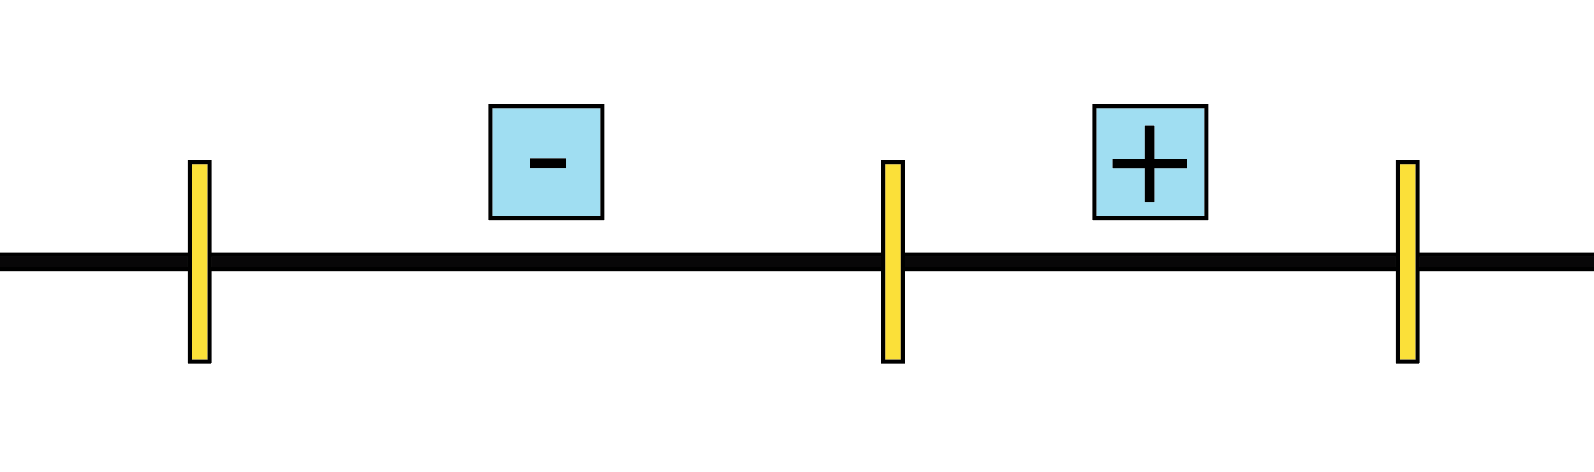
\includegraphics[width=0.5\textwidth]{assets/1_b.png}\] 
                
                \textit{t} can be put at any of the orange bars -- everything below is labeled as positive and everything above is negative. If the points are arranged as such and \textit{t} is at the leftmost position, + is categorized incorrectly. If it's at the middle position, both points are classified incorrectly, and if it's at the third point, then - is incorrectly classified. Therefore, $VC(\mathcal{H}) < 2$, or the upper bound is 2. 
                
                Additionally, VC has a minimum dimensionality of 1, so it cannot be 0, so the lower bound is 1. 
                
                Then, the VC dimensionality of the given example is \textbf{1}!
                
        \end{enumerate}
        
\end{enumerate}

\section{PAC Learning}
\begin{enumerate}
    \item 
    \begin{enumerate}
        \item Assuming that the same variable cannot be used on both the first and second level, there are 20 possible variables that can be used on the top layer of the tree and 19 possible variables that can be used on the bottom. 
        Then, the output of the tree has 
        \begin{equation*}
            2^4 
        \end{equation*}
        possible outputs since a Boolean is output from each of the nodes. 
        
        So, the number of structurally different trees can be computed: 
        \begin{equation*}
            20 * 19 * 2^4 = \text{6080 structurally different trees}
        \end{equation*}
        
        \item 
            The number \textit{m} can be computed with $\delta = .05$ and $\epsilon = .01$ as follows: 
            \begin{equation*}
                m > \frac{1}{\epsilon}(\ln{|H|} + \ln{\frac{1}{\delta}})
            \end{equation*}
            \begin{equation*}
                m > \frac{1}{0.01}(\ln{6080} + \ln{\frac{1}{0.05}}) = 1170.84922
            \end{equation*}
            \begin{equation*}
                m > 1170.8429
            \end{equation*}
            
            So, if you had 1171 (rounded up) examples, that would determine with probability .95 that we can learn a classifier whose accuracy is at least .99. 
            
        \item The following tree: 
        \[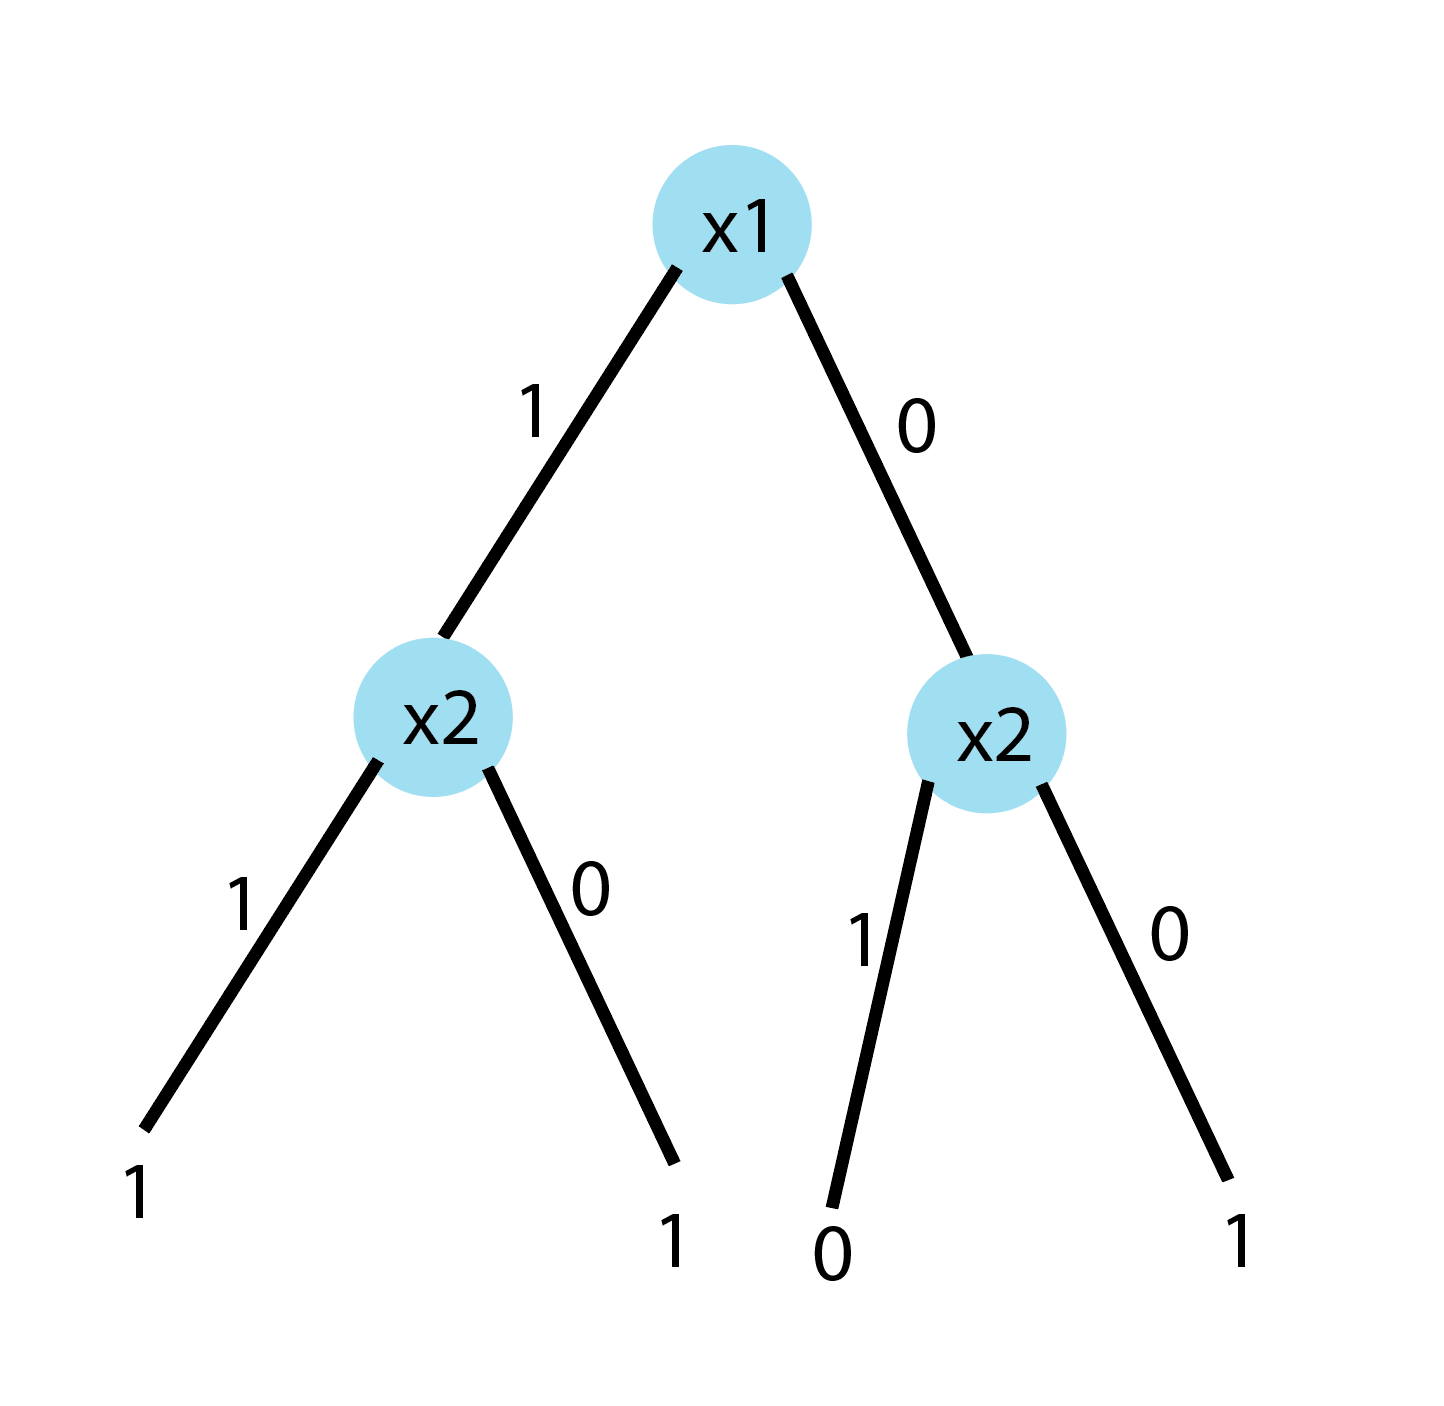
\includegraphics[width=0.5\textwidth]{assets/2_c_1.png}\] 
        
        Is functionally equivallent to the structurally different tree: 
        \[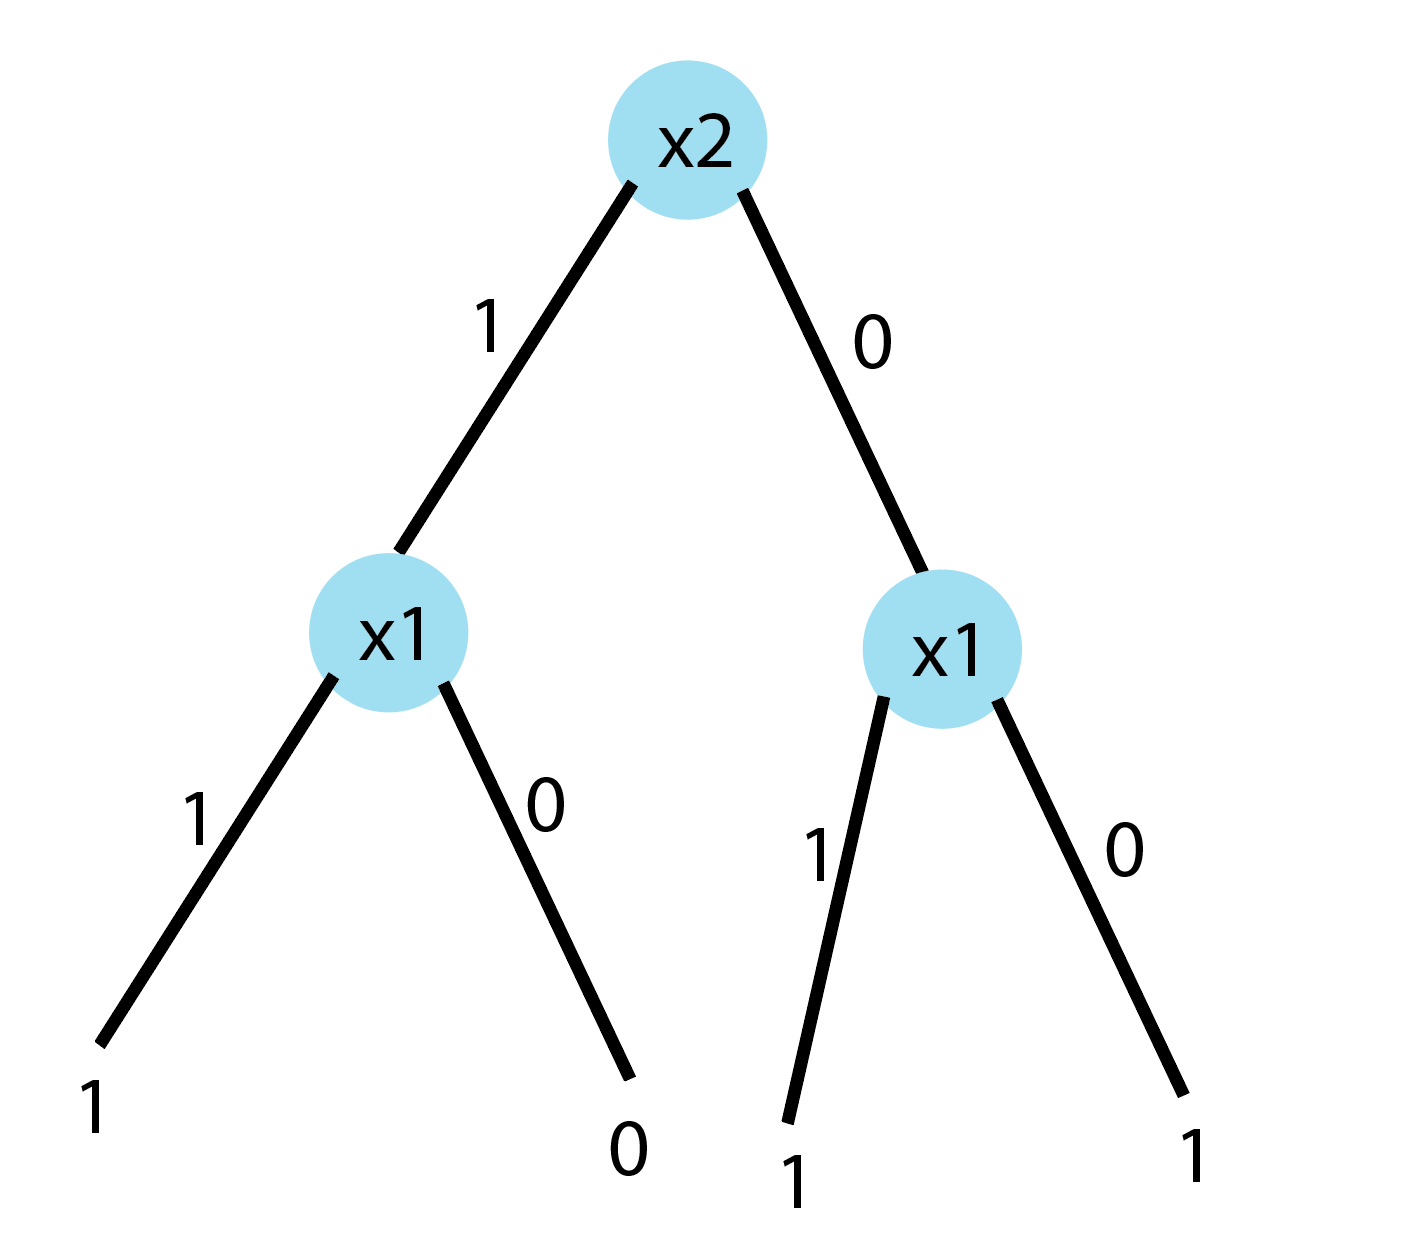
\includegraphics[width=0.5\textwidth]{assets/2_c_2.png}\] 
        
        This can be done with each tree in the set of structurally different trees, cutting the number of elements in the set in half! 
        
        \begin{equation*}
            \frac{6080}{2} = 3040
        \end{equation*}
        
    \end{enumerate}
        \item 
        \begin{equation*}
            m(\epsilon, \delta) = \frac{1}{\epsilon}(\ln{|H|} + \ln{\frac{1}{\delta}})
        \end{equation*}
        Given $\epsilon_1 \leq \epsilon_2 \leq 1$ and $\delta \in (0, 1)$, the claim $m(\epsilon_1, \delta) \geq m(\epsilon_2, \delta)$ can be proven as follows: 
        \begin{equation*}
            m(\epsilon_1, \delta) \geq m(\epsilon_2, \delta)
        \end{equation*}
        \begin{equation*}
            \frac{1}{\epsilon_1}(\ln{|H|} + \ln{\frac{1}{\delta}}) \geq \frac{1}{\epsilon_2}(\ln{|H|} + \ln{\frac{1}{\delta}})
        \end{equation*}
        \begin{equation*}
            \frac{1}{\epsilon_1} \geq \frac{1}{\epsilon_2}
        \end{equation*}
        \begin{equation*}
            \epsilon_2 \geq \epsilon_1
        \end{equation*}
        So, 
        \begin{equation*}
            m(\epsilon_1, \delta) \geq m(\epsilon_2, \delta) \textit{  QED}
        \end{equation*}
        
        
        Similarly, given $0 < \delta_1 \leq \delta_2 < 1$ and $\epsilon \in (0, 1)$, the claim 
        
        $m(\epsilon, \delta_1) \geq m(\epsilon, \delta_2)$ can be proven as follows: 
        \begin{equation*}
            \frac{1}{\epsilon}(\ln{|H|} + \ln{\frac{1}{\delta_1}}) \geq \frac{1}{\epsilon}(\ln{|H|} + \ln{\frac{1}{\delta_2}})
        \end{equation*}
        \begin{equation*}
            \ln{\frac{1}{\delta_1}} \geq \ln{\frac{1}{\delta_2}}
        \end{equation*}
        \begin{equation*}
            \frac{1}{\delta_1} \geq \frac{1}{\delta_2}
        \end{equation*}
        \begin{equation*}
            \delta_2 \geq \delta_1
        \end{equation*}
        So, 
        \begin{equation*}
            m(\epsilon, \delta_1) \geq m(\epsilon, \delta_2) \textit{  QED}
        \end{equation*}
        
\end{enumerate}

\section{VC Dimension}

\begin{enumerate}
    \item 
    \begin{enumerate}
        \item
            The most \textit{adversarial} (so to speak, for this problem) ordering of four points is as follows: 
            \[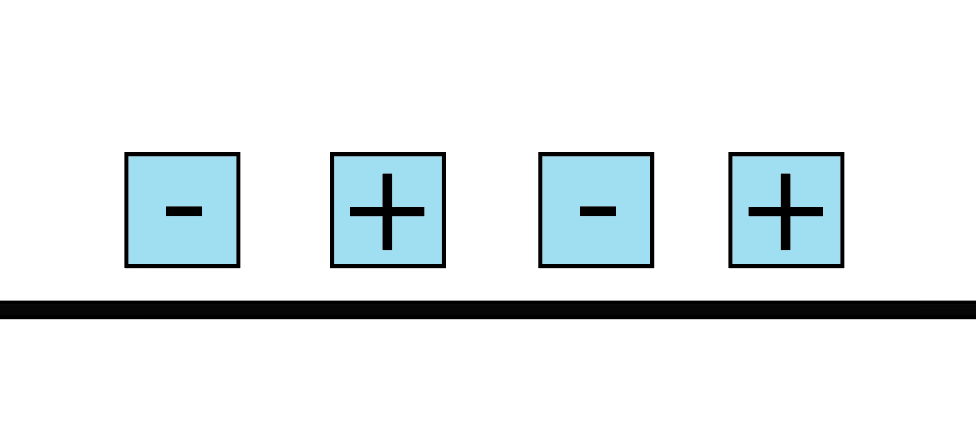
\includegraphics[width=0.5\textwidth]{assets/3_1_a.png}\]
            \textit{Or some orientation of alternating points.} 
            
            There can be two regions marked as positive -- and since the positive points are separated there will be two positive regions needed to label all points correctly. Two positive labels separated can always be classified correctly. 
            
            In the case that there are no positive labels, the two positive regions can be placed at arbitrary points such that they don't encapsulate any negative points and everything will still be classified correctly. 
            
            Similarly, in the case where there's one positive label and three negative labels, a positive region can be used to isolate the single positive point and the other can be placed at an arbitrary location such that it doesn't isolate any negative points. 
            
            Since all the points are in a line, if there are more than two positive points, two or more of those points can be placed together in the same group. 
            
            Therefore, the lower bound of VC($\mathcal{H}$) is 4, and we can determine that $\text{VC}(\mathcal{H}) \geq 4$. 
            
        \item 
            Similarly to above, the most \textit{adversarial} (so to speak, for this problem) organization of points with five points is as follows: 
            \[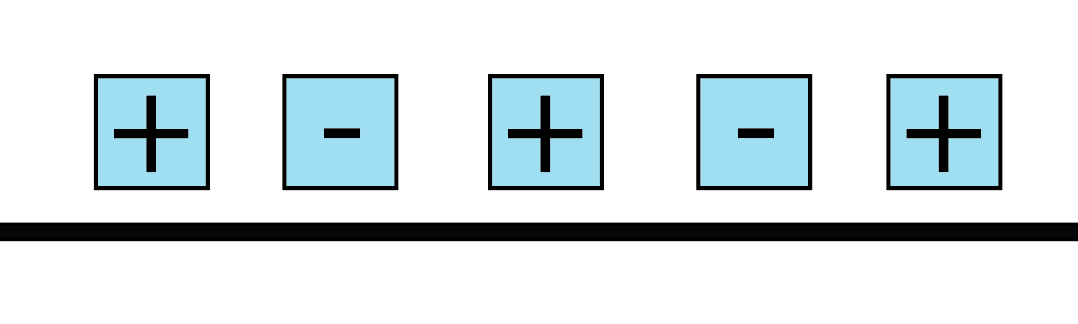
\includegraphics[width=0.5\textwidth]{assets/3_1_b.png}\]
            
            Where there are three isolated positive points. Since there's only two given regions that are positive, there is no orientation of these regions such that they isolate all three positive points -- this orientation of points cannot be shattered and therefore sets an upper bound of VC($\mathcal{H}$) = 5, or: $\text{VC}(\mathcal{H}) < 5$
            
            So,
            
            \begin{equation*}
                VC(\mathcal{H}) = 4
            \end{equation*}

    \end{enumerate}
    
    \item 
        Graduate students only. 
    
    \item 
        To \textit{prove the lower bound} on $VC(\mathcal{H})$, assume five points are placed in a pentagonal pattern as such: 
        \[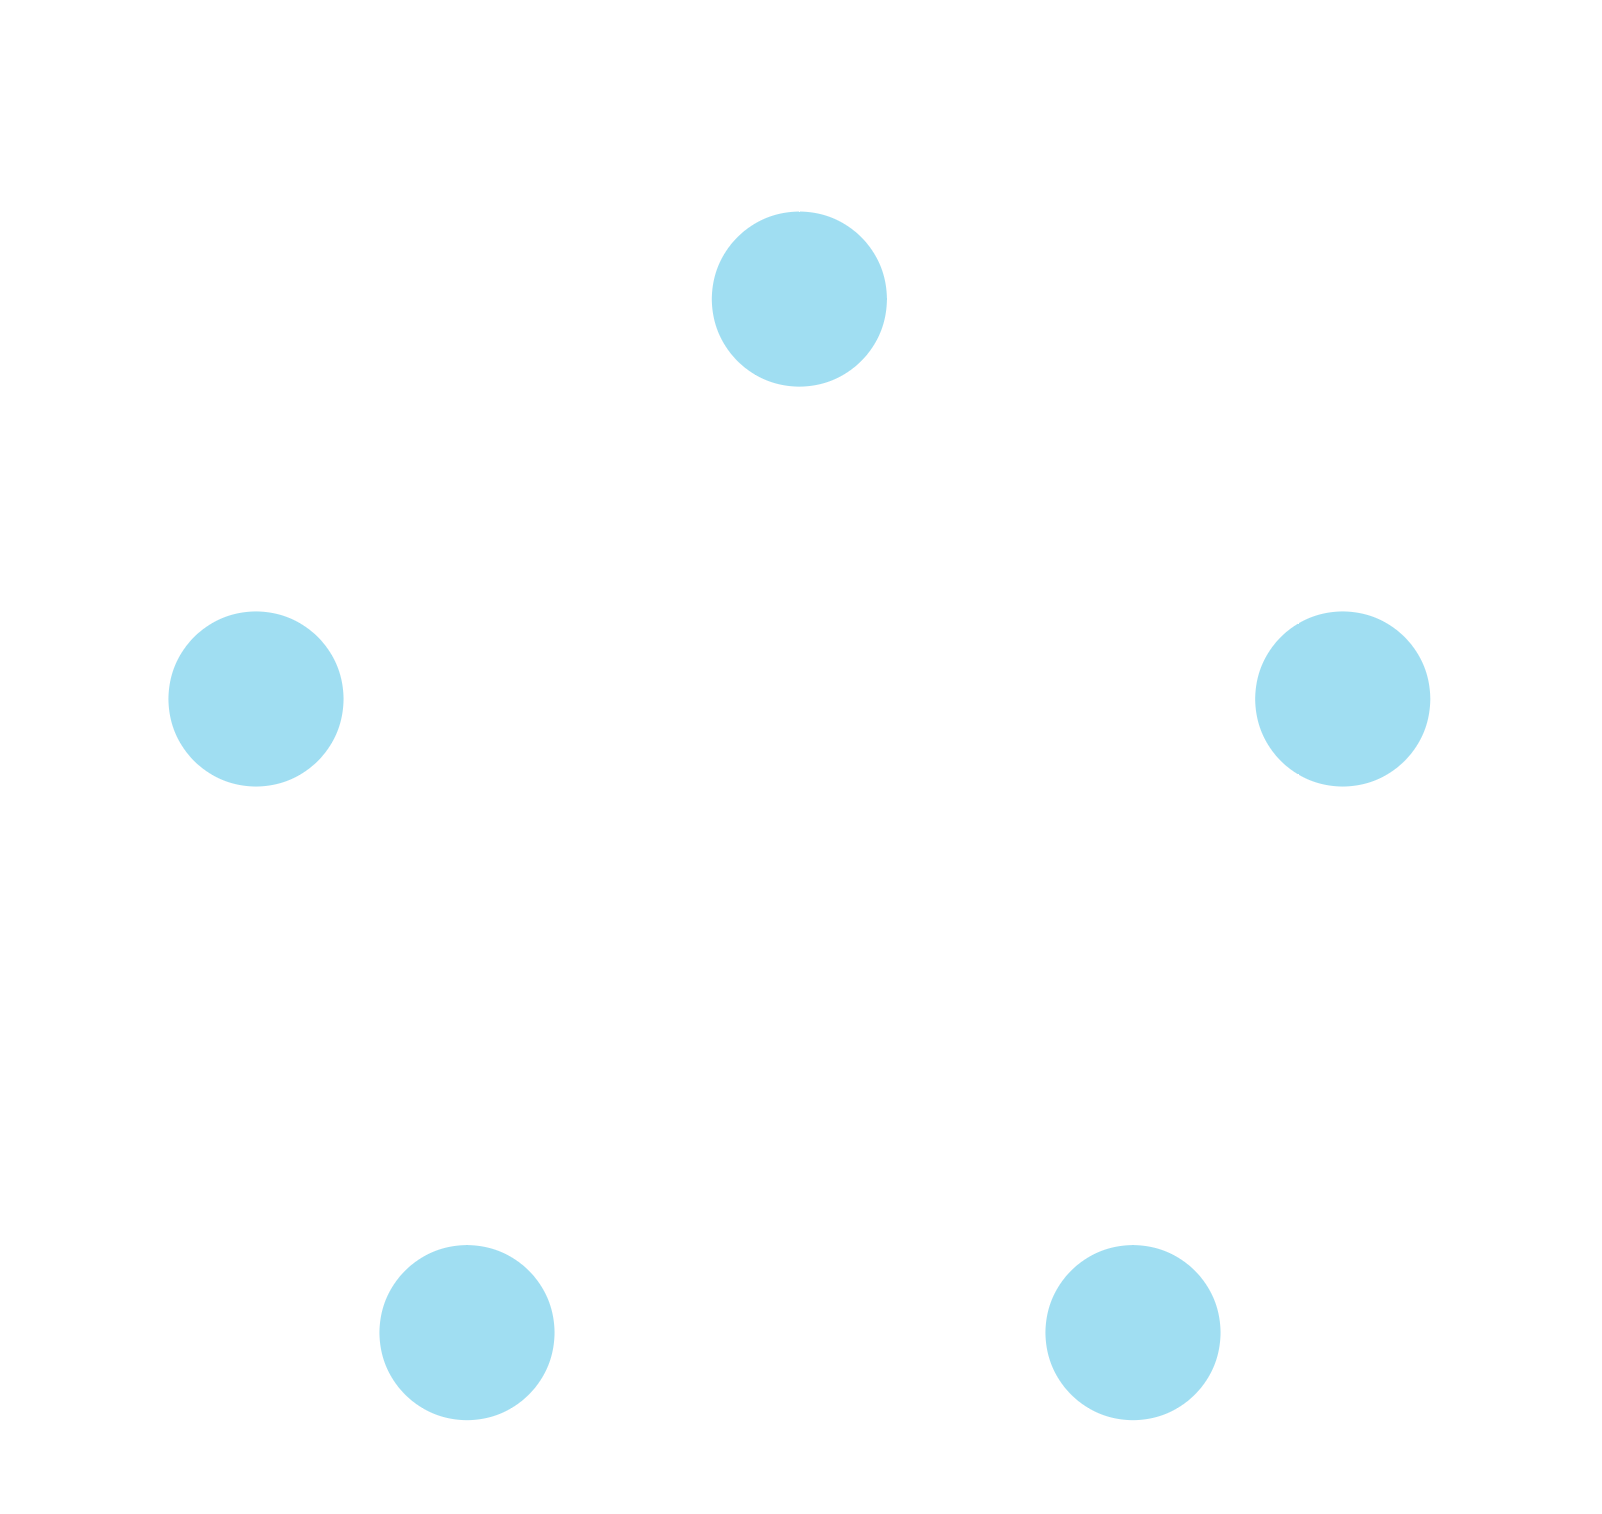
\includegraphics[width=0.5\textwidth]{assets/3_3.png}\] 
        
        There are $2^5 = 32$ possibilities of point combinations. I went through all of them, and there are no points that exist such that two parallel lines cannot correctly separate any combination of these points. I'll save you from going 32 images, so here's the gist: 
        
        \textbf{Zero + Points: } The parallel lines can be placed any arbitrary position such that they don't overlap the negative points. 
        
        \textbf{One + Point: } A single positive point can always be separated from four negative points as no points are colinear: 
        \[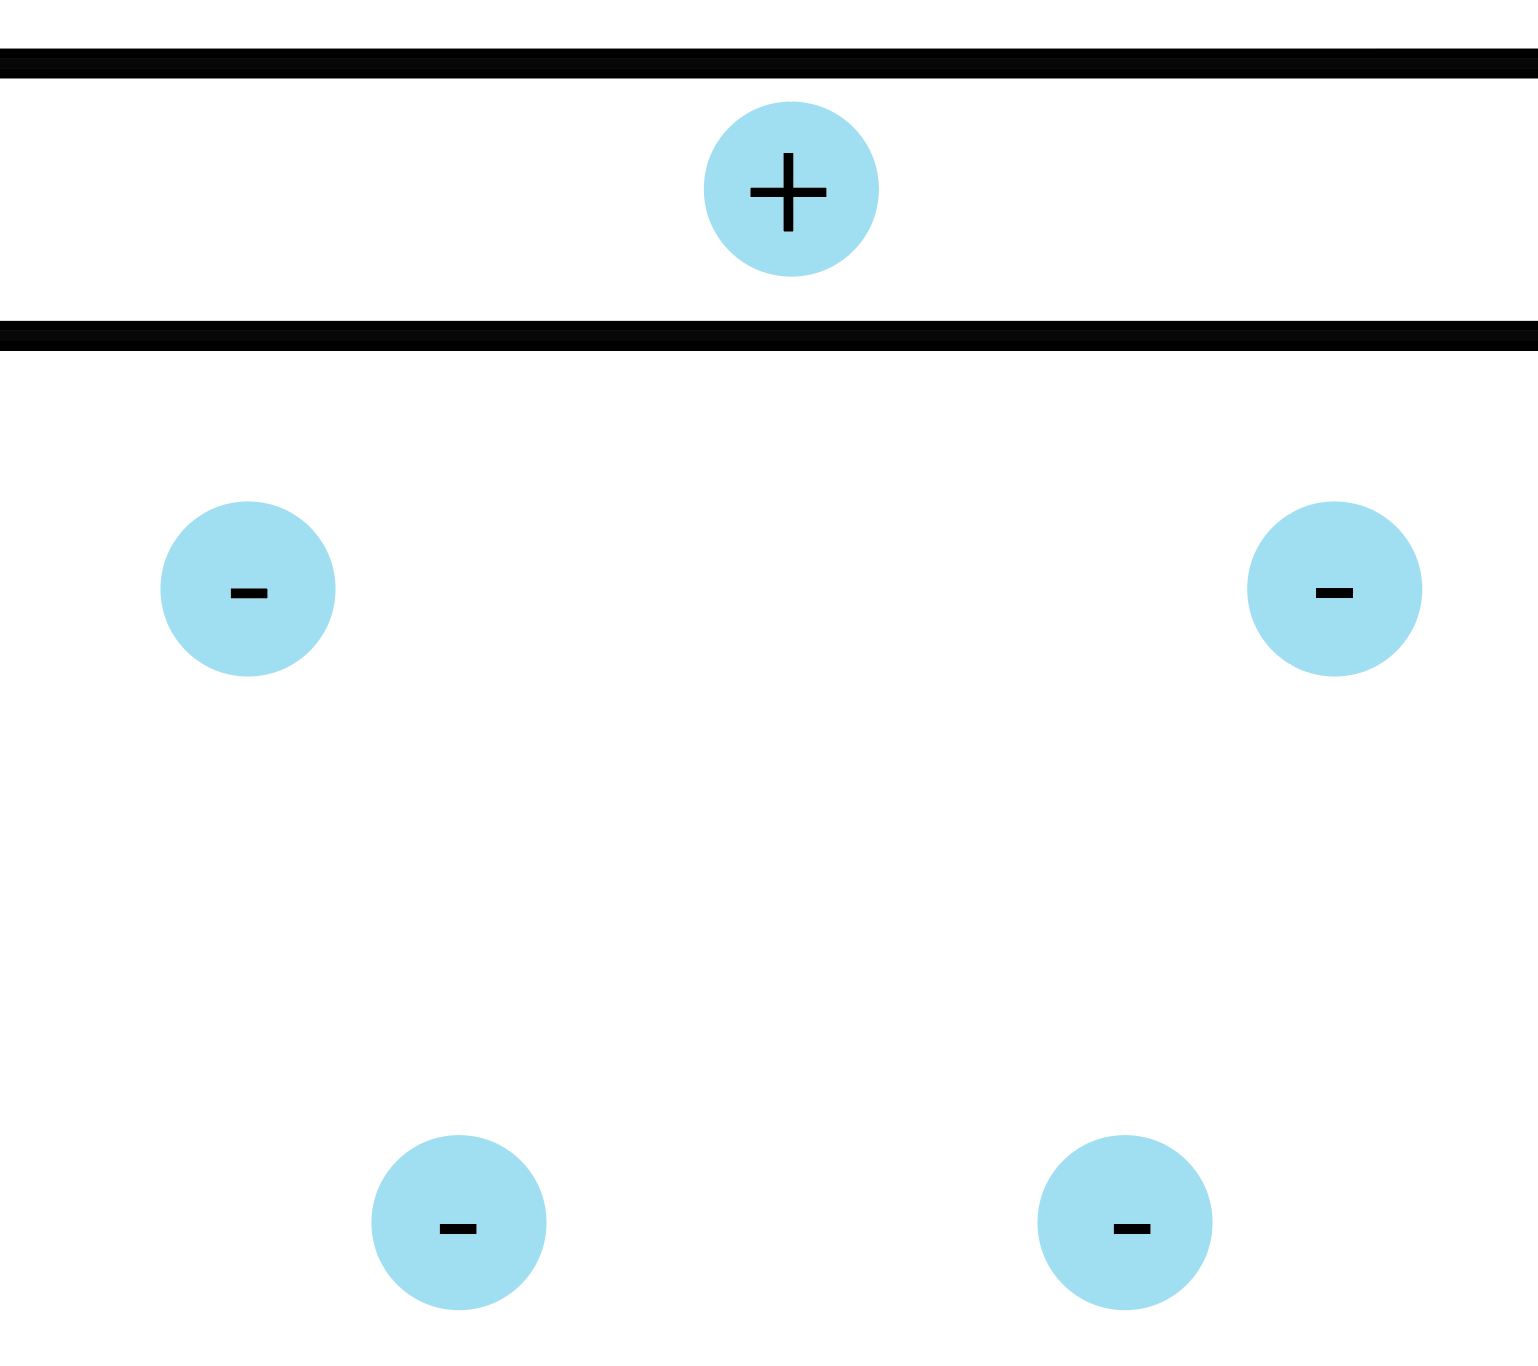
\includegraphics[width=0.5\textwidth]{assets/3_3_3.png}\] 
        
        \textbf{Two + Points: } Take, for example, the following combination of points and its separator: 
        \[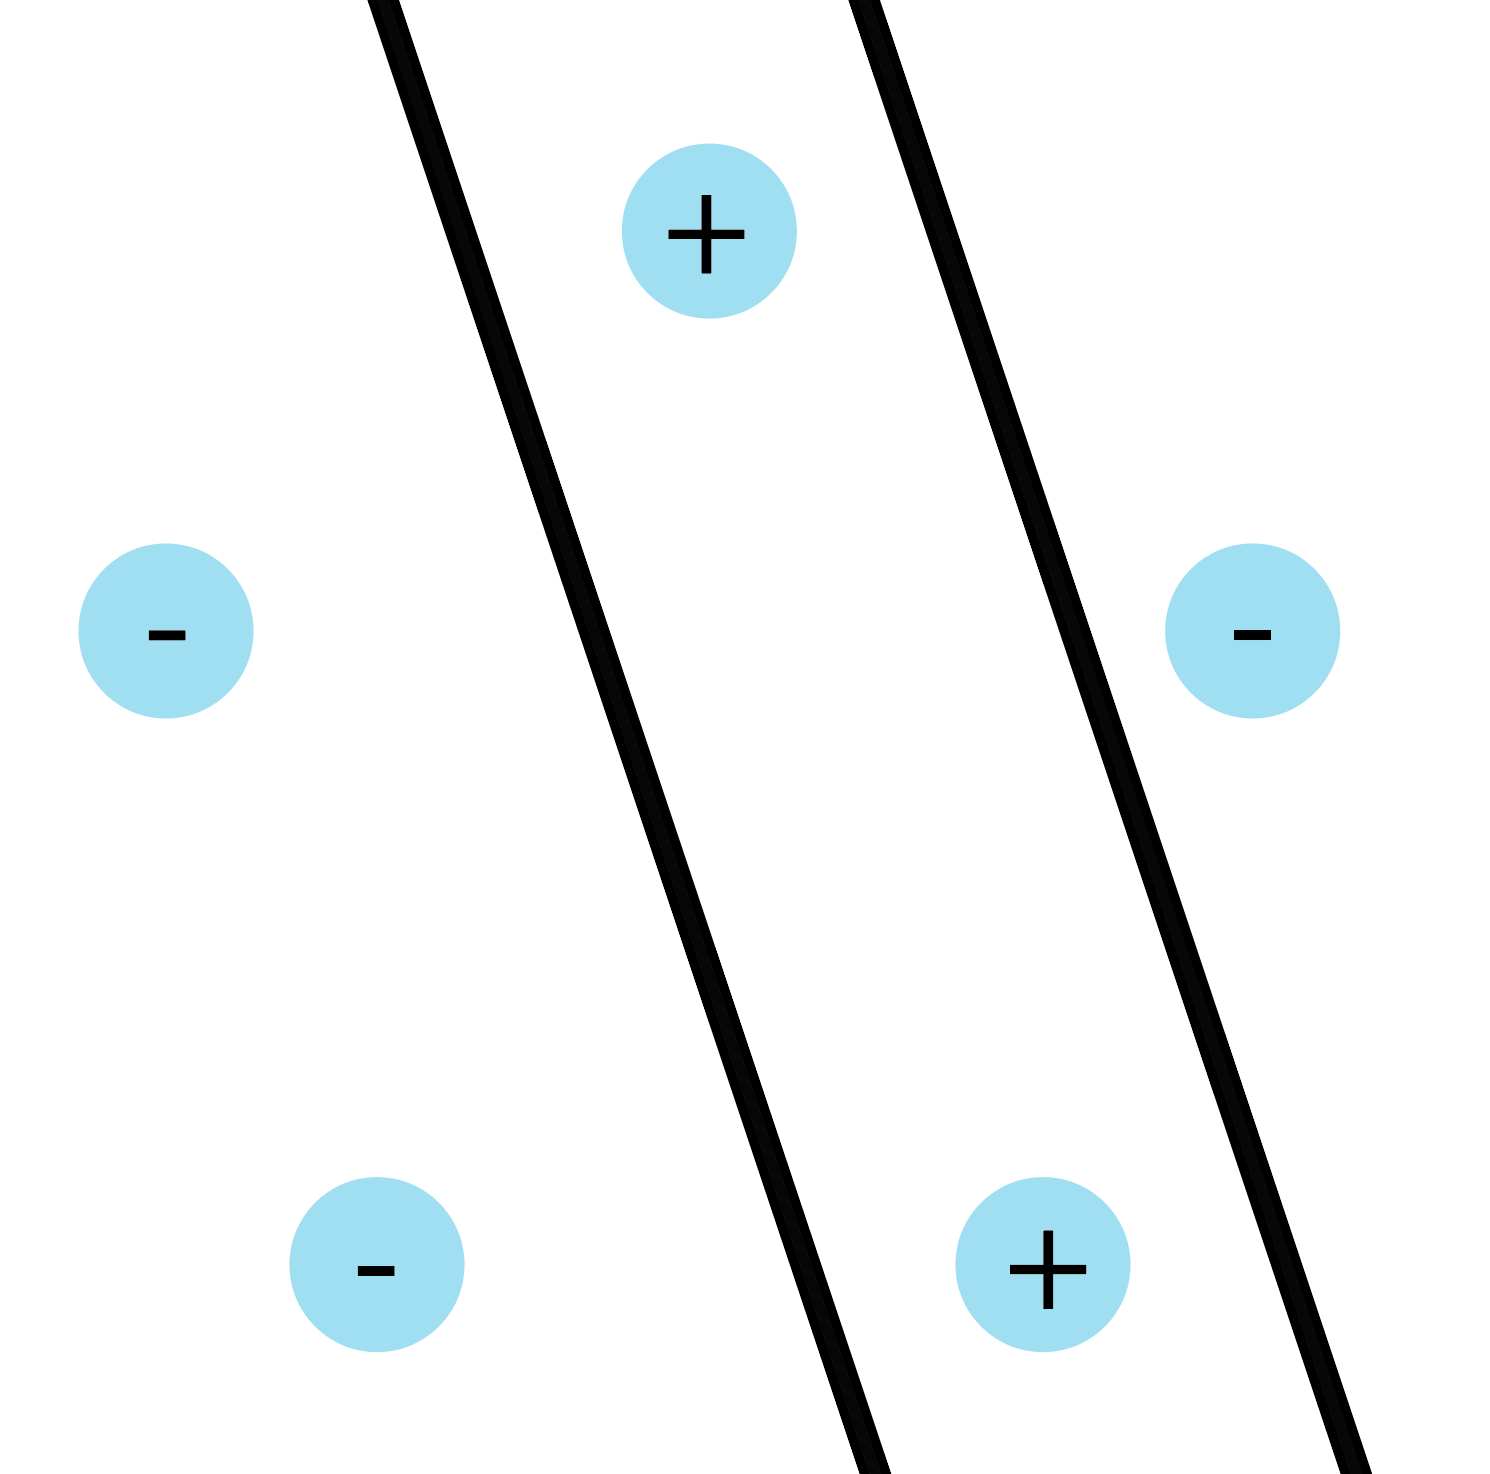
\includegraphics[width=0.5\textwidth]{assets/3_3_2.png}\] 
        
        By simply rotating the lines as needed, any combination of two positive points can be separated from the negative points. 
        
        \textbf{Three + Points: } 
        In the same way that \textit{Two + Points} can be isolated, do the same to the negative points and leave them out of the section that classifies the + points. 
        
        \textbf{Four + Points: }
        Opposite to \textit{One + Point}, the - point can be isolated from the rest of the points because none of the points are colinear and can all be separated from each other. 
        \[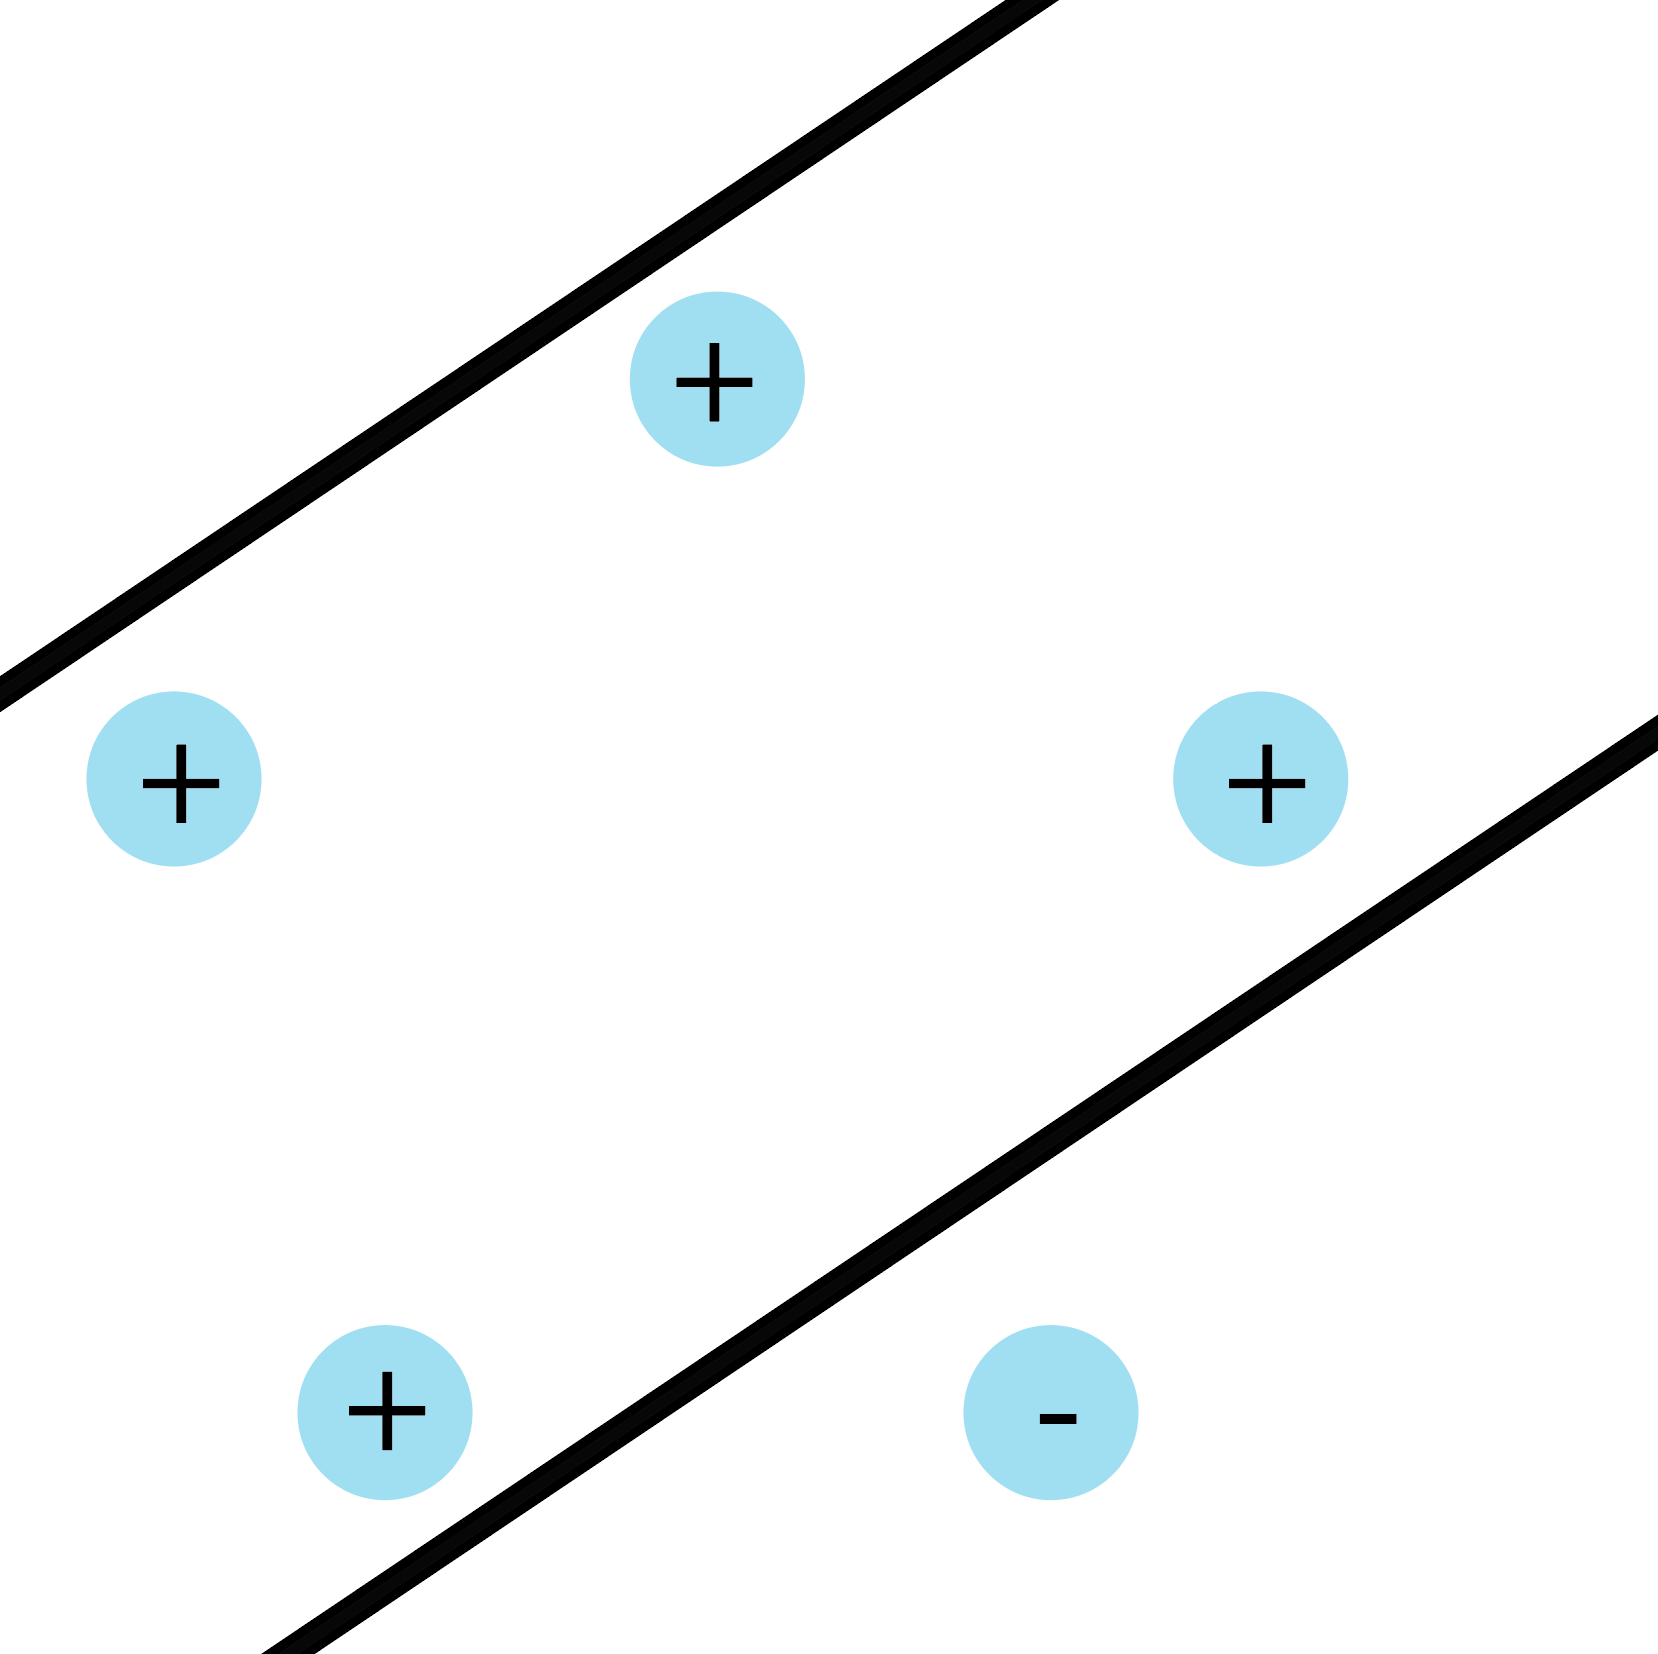
\includegraphics[width=0.5\textwidth]{assets/3_3_4.png}\] 
        
        \textbf{Five + Points: }
        Opposite to \textit{Zero + Points}, place the lines around the points to encompass all of them. 
        
        Therefore the lower bound of $VC(\mathcal{H})$ is 5, and we can determine that $VC(\mathcal{H}) \geq 5$. 
        
        To \textit{prove the upper bound} on $VC(\mathcal{H})$, say that the points were arranged in a 6-sided polygon: 
        \[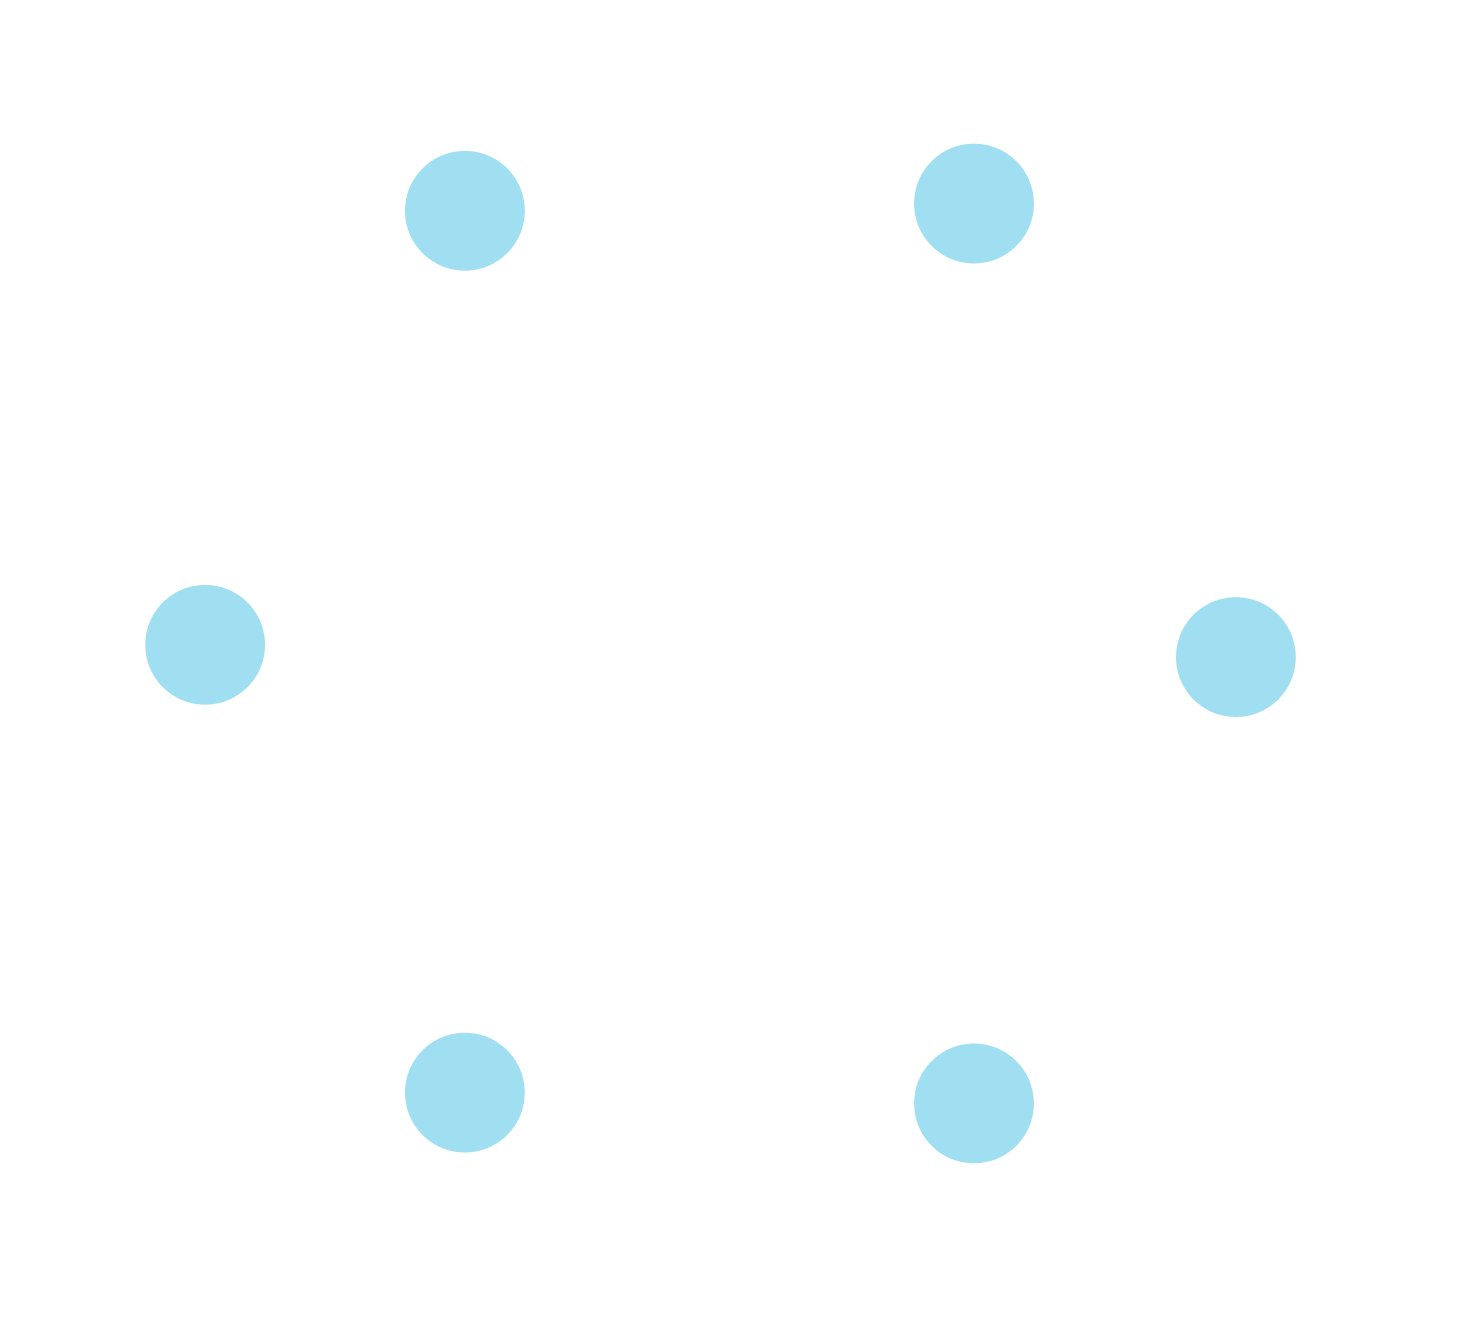
\includegraphics[width=0.5\textwidth]{assets/3_3_5.png}\] 
        
        Further, say that the points were arranged as thus: 
        \[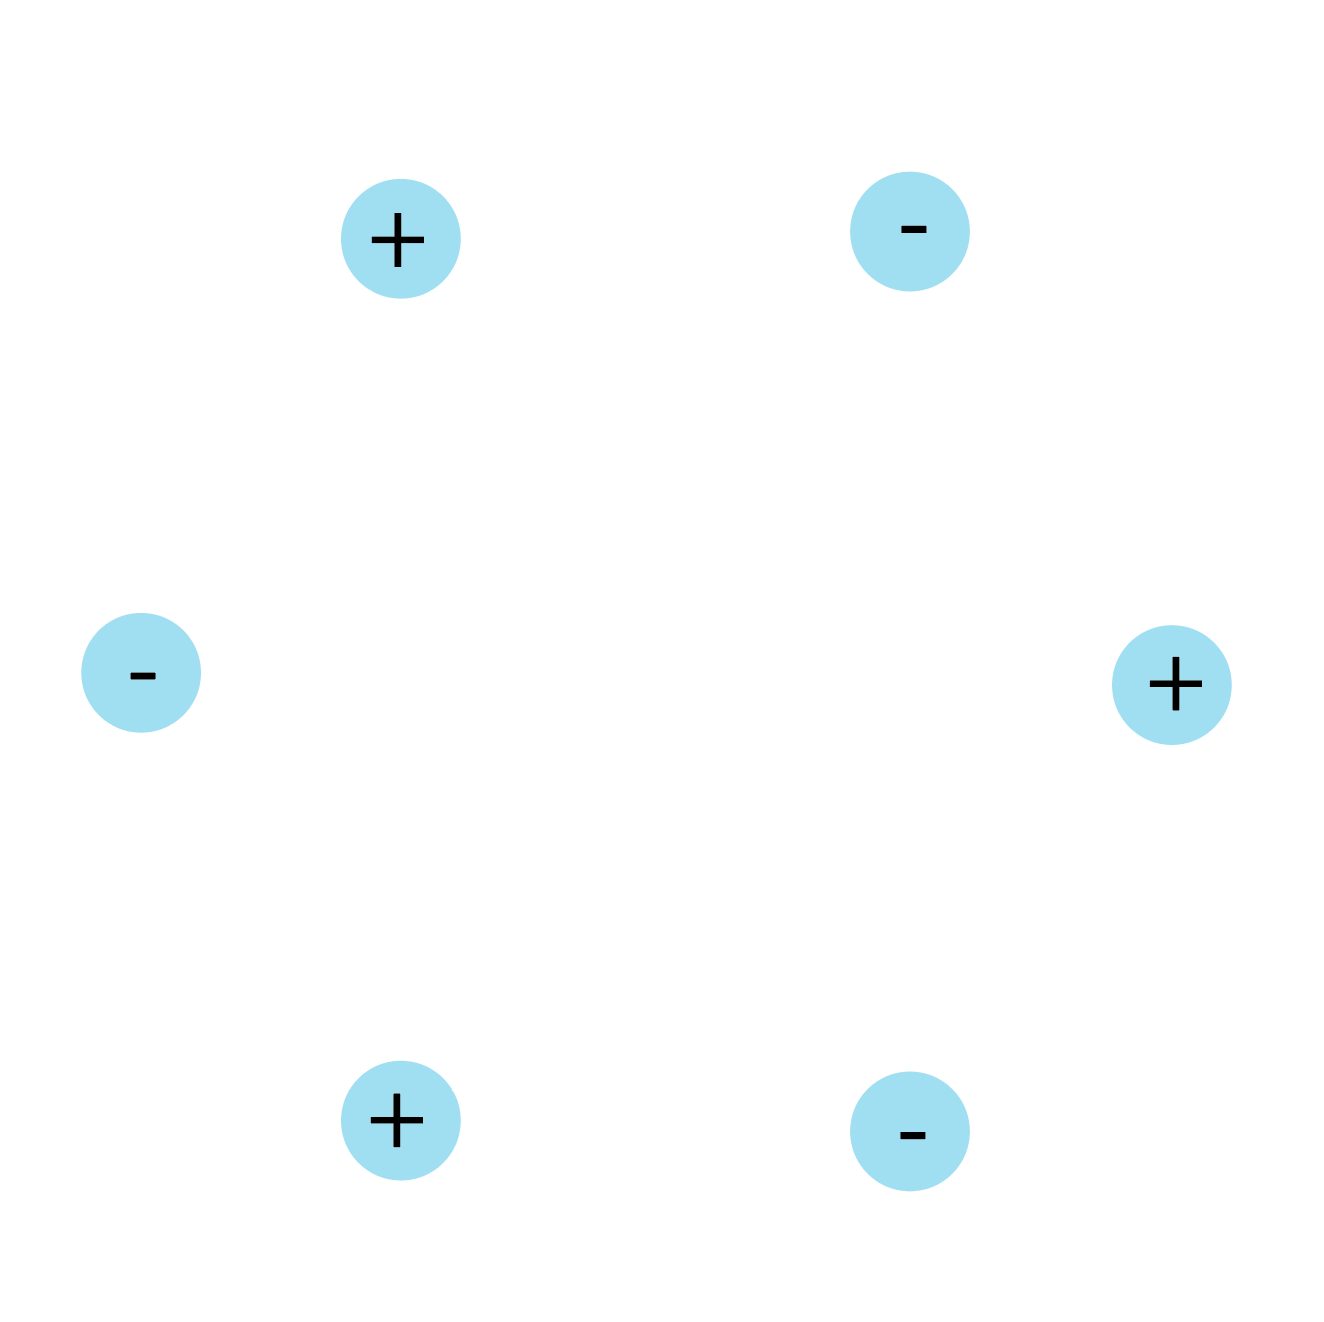
\includegraphics[width=0.5\textwidth]{assets/3_3_6.png}\] 
        
        Since a six-sided polygonal arrangement introduces colinear points, this arrangement cannot be shattered. The best that one could do is something like the following: 
        \[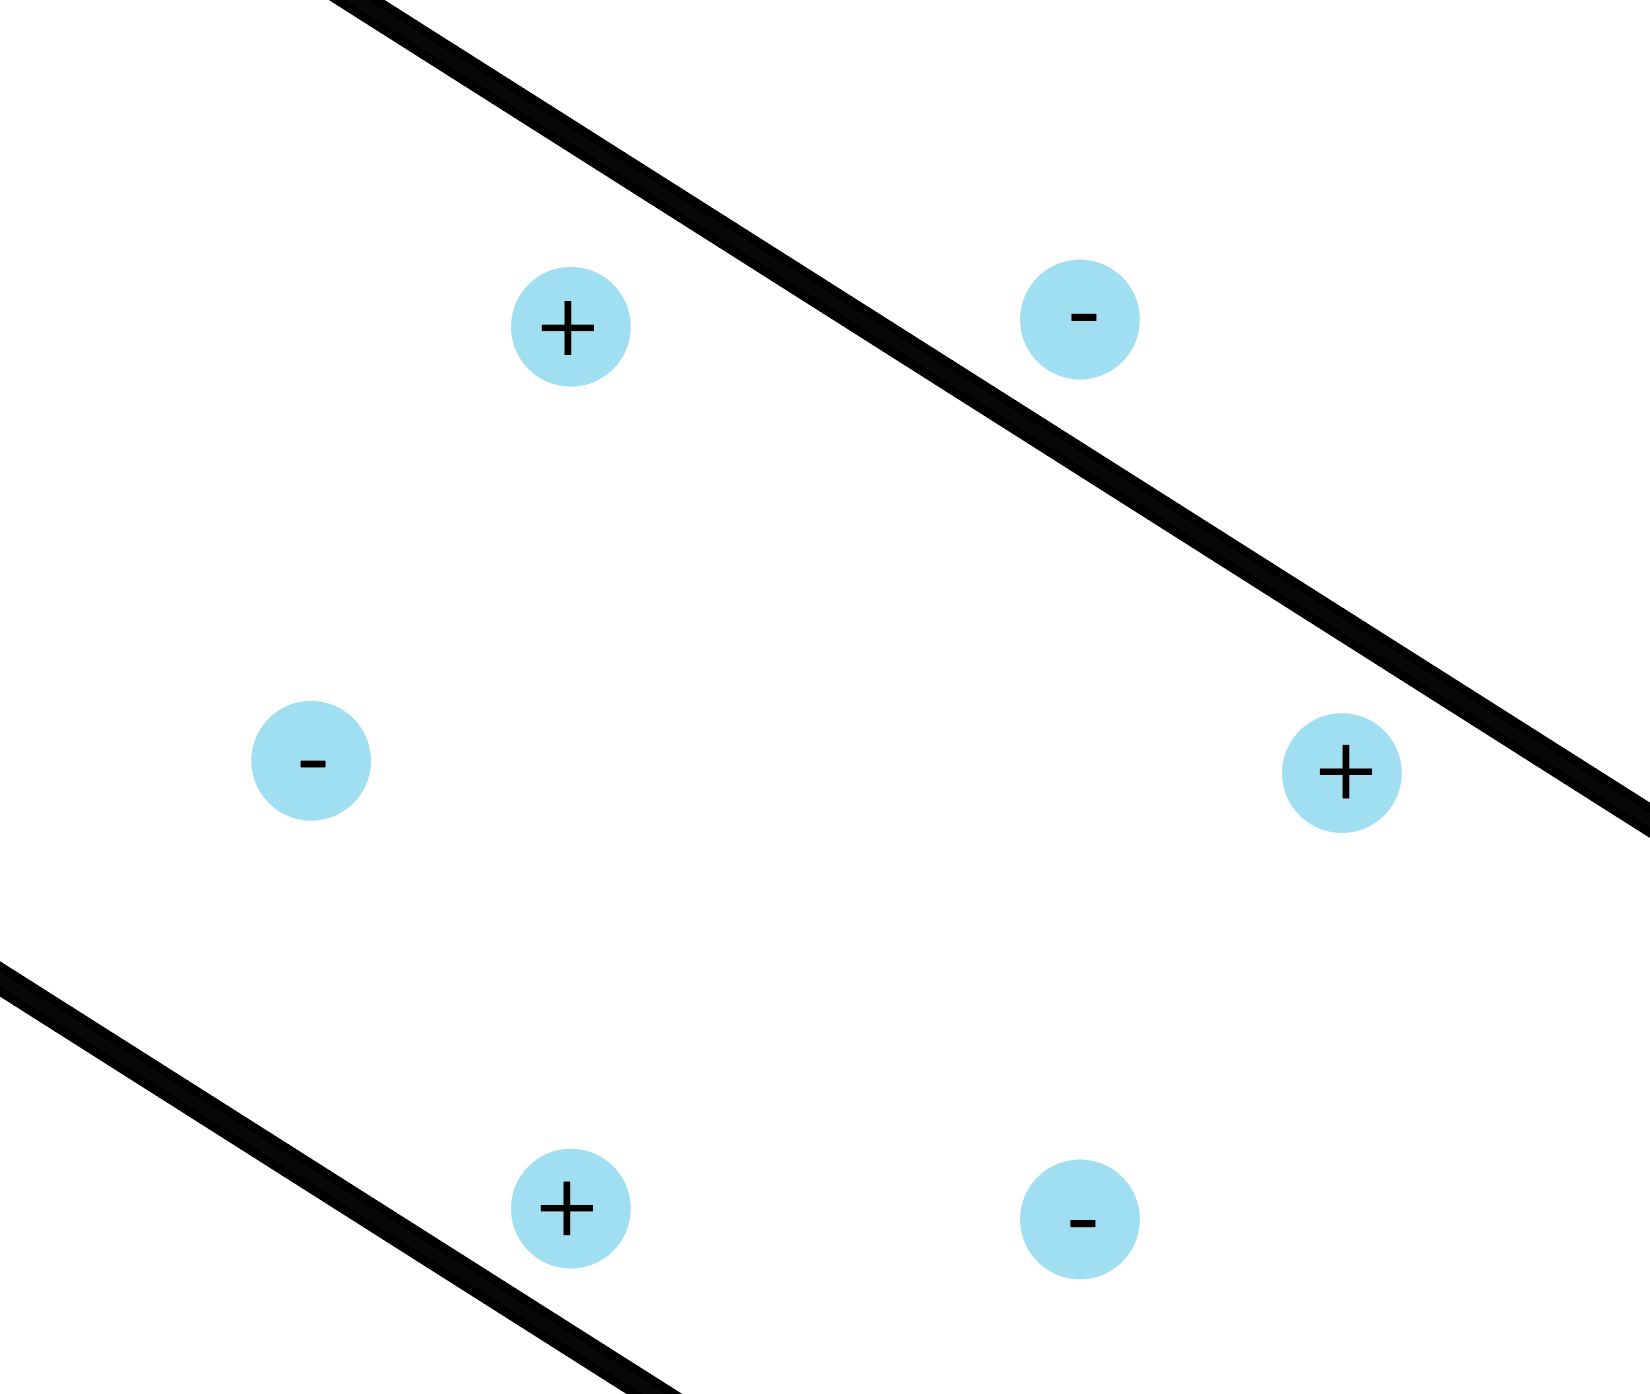
\includegraphics[width=0.5\textwidth]{assets/3_3_7.png}\] 
        
        But, this classifies points incorrectly. That's because, with the colinearity introduced on the top and bottom of the polygon, essentially two triangles are created between the shapes and it makes it so they cannot be separated using a threshold made by two lines. The points make a convex hull -- and this is required for the linear separation above -- but again because of the colinearity introduced by the polygonal shape, the points cannot be always shattered and the above is an example of that. Some version of the above will be true for some arrangement of six points in arbitrary space, too. Adding more points, of course, makes the problem more complex but since $\mathcal{H}$ stays the same, the more points you add the more combinations of those points something in $\mathcal{H}$ cannot shatter. 
        
        As such, the upper bound of $VC(\mathcal{H})$ is 6. 
        
        So,
        \begin{equation*}
            VC(\mathcal{H}) = 5
        \end{equation*}  
    
    \item 
        To prove that if $\mathcal{H} \subseteq \mathcal{G} \text{  then   } VC(\mathcal{H}) \leq VC(\mathcal{G})$, let's assume that $VC(\mathcal{H}) > VC(\mathcal{G})$. 
        
        This requires that H contains a function that is not present in $\mathcal{G}$, as we are able to shatter more sets of points with $\mathcal{H}$. 
        
        However, we're given that $\mathcal{H} \subseteq \mathcal{G}$, therefore $\mathcal{H}$ cannot contain any functions not in $\mathcal{G}$. 
        
        This is a contradiction. 
        
        It is impossible for $VC(\mathcal{H}) > VC(\mathcal{G})$ as the concept class $\mathcal{G}$ has more information than $\mathcal{H}$. $\mathcal{H}$ cannot be more expressive than $\mathcal{G}$ because it has less information. 
        
        Therefore via proof by contradiction, $VC(\mathcal{H}) \leq VC(\mathcal{G})$ if $\mathcal{H} \subseteq \mathcal{G}$. 
        
        \textit{QED}.
        
    \item 
        Given that $\mathcal{H}$ is a finite concept class, if $VC(\mathcal{H}) = d$ then $|\mathcal{H}| \geq 2^d$. This can be proven as follows: 
        
        Assume that if $|\mathcal{H}| < 2^{VC(\mathcal{H})}$ then there is some hypothesis unaccounted for. This would mean that $\mathcal{H}$ cannot shatter $d$ points. 
        
        However, we're given that $\mathcal{H}$ \textit{can} shatter $VC(\mathcal{H}) = d$ points. 
        
        So, 
        
        \begin{equation*}
            |H| \geq 2^{VC(\mathcal{H})} = 2^d 
        \end{equation*}
        
        Were this not the case, some hypothesis would have to satisfy shattering multiple labelings, which is not possible. One hypothesis in $\mathcal{H}$ does not provide enough information to shatter multiple point sets. A unique hypothesis is needed for each unique labeling of points in the data set, and were it the case that there were less hypotheses than point placements, not all arrangements could be shattered. 
        
        Therefore via proof by contradiction, given $VC(\mathcal{H}) = d$ then $|\mathcal{H}| \geq 2^d$.
        
        \textit{QED.}
\end{enumerate}

        
\end{document}
